\FloatBarrier
\subsection{Evaluation}
\label{sec:hard_cut_evaluation}




The SVM is trained on an mixture of videos from the 2007 TrecVid contest.
The videos in their full length do not make a good training set, as the ratio between hard cuts and other frames is about \texttt{1:1000}, leading to a failure to predict any hard-cuts.
A custom training set must be constructed, which contains a suffcient amount of hard cuts.
The choice of non-hard-cuts is also crucial for achieving good classification performance: too homogenous frames will lower the decision boundary, and lead to bad performance on noisy examples.
Therefore the negative set should also include soft-cuts and particularly noisy frames.
The training set we finally build consists of about 250 hard cuts and 2200 negatives.


We evaluate our approach on complete, heldout videos of the 2007 TrecVid contest. The results per video are shown in Figure~\ref{fid:scatterplothceval}, showing that a high recall is consistently achieved, while the precision is dependent on the video. The overall statistic, shown in Table~\ref{tab:hard_cut_results},  reveals that the objective of further improvements must be to reduce the number of false positives.

\begin{figure}
\centering
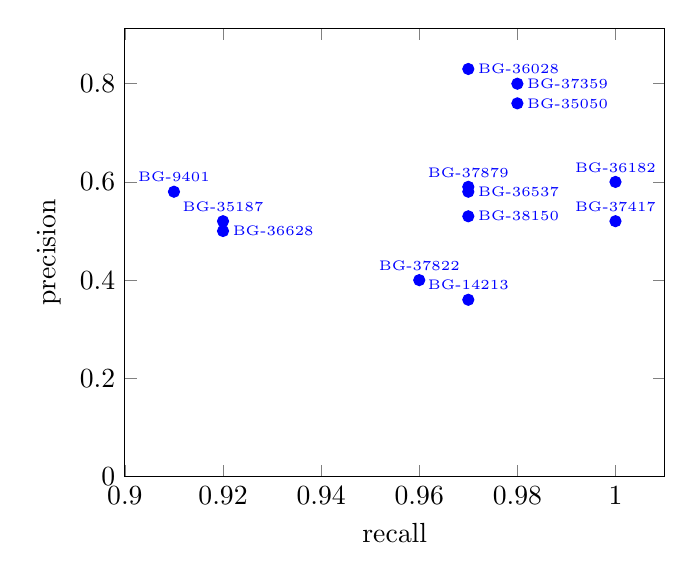
\begin{tikzpicture}
\begin{axis}[
	domain=0:1.0,
	ymin=0.0, xmin = 0.9,
    ylabel=precision,
    xlabel=recall
]


\addplot[blue,mark=*,mark options={fill=blue},nodes near coords,only marks,
   point meta=explicit symbolic, visualization depends on={value \thisrow{anchor}\as\myanchor},
   every node near coord/.append style={anchor=\myanchor,font=\tiny}] table[meta=label] {
x y label anchor
0.97 0.36  BG-14213 south
0.98 0.76  BG-35050 west
0.92 0.52   BG-35187 south
0.97 0.83   BG-36028 west
1    0.6   BG-36182 south
0.97 0.58  BG-36537 west
0.92 0.5   BG-36628 west
0.98 0.8   BG-37359 west
1    0.52  BG-37417 south
0.96 0.4   BG-37822 south
0.97 0.59  BG-37879 south
0.97 0.53  BG-38150 west
0.91 0.58  BG-9401 south
};
\end{axis}
\end{tikzpicture}
\caption{Results on TrecVid 2007 Videos}
\label{fid:scatterplothceval}
\end{figure}

%Complete Results, for reference
% BG_14213
% TP: 103 FP: 184 TN: 82821 FN: 3
% Precision: 0.36
%    Recall: 0.97
%        F1: 0.52
% BG_35050
% TP: 96 FP: 30 TN: 36867 FN: 2
% Precision: 0.76
%    Recall: 0.98
%        F1: 0.86

%  BG_35187
% TP: 124 FP: 116 TN: 28770 FN: 11
% Precision: 0.52
%    Recall: 0.92
%        F1: 0.66

% BG_36028
% TP: 84 FP: 17 TN: 44883 FN: 3
% Precision: 0.83
%    Recall: 0.97
%        F1: 0.89

% BG_36182
% TP: 95 FP: 64 TN: 29447 FN: 0
% Precision: 0.6
%    Recall: 1
%        F1: 0.75

% BG_36537
% TP: 251 FP: 181 TN: 49560 FN: 8
% Precision: 0.58
%    Recall: 0.97
%        F1: 0.73

% BG_36628
% TP: 177 FP: 174 TN: 56195 FN: 15
% Precision: 0.5
%    Recall: 0.92
%        F1: 0.65

% BG_37359
% TP: 160 FP: 40 TN: 28700 FN: 4
% Precision: 0.8
%    Recall: 0.98
%        F1: 0.88

% BG_37417
% TP: 76 FP: 70 TN: 22854 FN: 0
% Precision: 0.52
%    Recall: 1
%        F1: 0.68
%  Accuracy: 1

% BG_37822
% TP: 114 FP: 174 TN: 21663 FN: 5
% Precision: 0.4
%    Recall: 0.96
%        F1: 0.56
%  Accuracy: 0.99

% BG_37879
% TP: 92 FP: 63 TN: 28857 FN: 3
% Precision: 0.59
%    Recall: 0.97
%        F1: 0.74
%  Accuracy: 1


% BG_38150
% TP: 208 FP: 187 TN: 52244 FN: 7
% Precision: 0.53
%    Recall: 0.97
%        F1: 0.68
%  Accuracy: 1

% BG_9401
% Evaluating on 89/50045 positive instances.
% TP: 81 FP: 58 TN: 49898 FN: 8
% Precision: 0.58
%    Recall: 0.91
%        F1: 0.71
%  Accuracy: 1


\begin{table}[ht]
	\centering
	\begin{tabular}{l|l|l||l|l|l|l}
	Precision & Recall & F1 & TP & FP & TN & FN \\ \hline
	0.55 \% & 0.96 \% & 0.7 \% & 1661 & 1358 & 532759 & 69 \\ 
	\end{tabular}

	\caption{Results on complete 2007 TrecVid dataset}
	\label{tab:hard_cut_results}
\end{table}

